\begin{frame}
\frametitle{Swarm}
\framesubtitle{Overview}
Multiple Docker hosts can be managed in a centralized manner using an inner feature of Docker: \textbf{\textit{Swarm}}
\end{frame}

\begin{frame}
\frametitle{Swarm}
\framesubtitle{Overview}
\begin{itemize}
\item Cluster management
\item Decentralized design (one is all)
\item Declarative service model
\item Scaling
\item Desired state reconciliation
\item Multi-host networking
\item Service discovery
\item Load balancing
\item Secure by default (TLS)
\item Rolling updates
\end{itemize}
\end{frame}

\begin{frame}
\frametitle{Swarm}
\framesubtitle{Overview}
A generic Docker Host is a \textit{Node} in the Swarm.
\end{frame}

\begin{frame}
\frametitle{Swarm}
\framesubtitle{Overview}
A generic Docker Host is a \textit{Node} in the Swarm.\\
\vspace{0.4cm}
A Node can be:
\begin{itemize}
\item Manger: dispatches tasks to workers; orchestrates and manages the cluster
\item Worker: executes a task  
\end{itemize}
\end{frame}

\begin{frame}
\frametitle{Swarm}
\framesubtitle{Overview}
A \textit{Service} is the formal definition of a Task.\\
\vspace{0.4cm}
A \textit{Task} is the instance of a Service.
\end{frame}

\begin{frame}
\frametitle{Swarm}
\framesubtitle{Overview}
\begin{center}
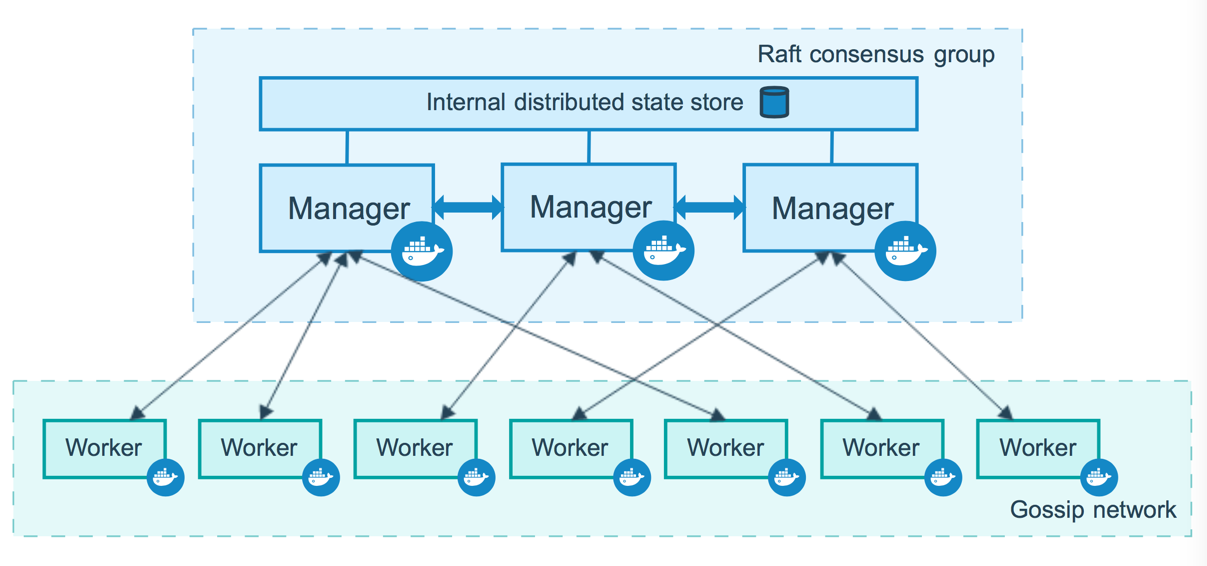
\includegraphics[width=\columnwidth]{./Figure/swarm-diagram}
\end{center}
\end{frame}

\begin{frame}
\frametitle{Swarm}
\framesubtitle{Setup}
You can create a Swarm environment using \href{https://www.virtualbox.org/wiki/Downloads}{VirtualBox}
\vspace{0.4cm}
\begin{itemize}
\item \href{https://download.virtualbox.org/virtualbox/6.0.8/VirtualBox-6.0.8-130520-Win.exe}{Windows}
\item \href{https://download.virtualbox.org/virtualbox/6.0.8/VirtualBox-6.0.8-130520-OSX.dmg}{OS X}
\item \href{https://www.virtualbox.org/wiki/Linux_Downloads}{Lilnux}
  \begin{itemize}
    \item \href{https://download.virtualbox.org/virtualbox/6.0.8/virtualbox-6.0_6.0.8-130520~Ubuntu~bionic_amd64.deb}{Ubuntu}
    \item \href{http://dl-cdn.alpinelinux.org/alpine/v3.9/releases/x86_64/alpine-virt-3.9.4-x86_64.iso}{AlpineLinux}
  \end{itemize}
\end{itemize}
\end{frame}


\begin{frame}[fragile]
\frametitle{Swarm}
\framesubtitle{Setup: VirtualBox}
\begin{lstlisting}
VBoxManage natnetwork add 
  --netname swarm 
  --network "192.168.15.0/24" 
  --enable --dhcp on
\end{lstlisting}
\tiny
\href{https://www.virtualbox.org/manual/ch06.html#network_nat_service}{VirtualBox NAT service}
\normalsize
\end{frame}


\begin{frame}
\frametitle{Swarm}
\framesubtitle{Setup: Virtual Machine}
Create a virtual machine with default parameters
\end{frame}

\begin{frame}[fragile]
\frametitle{Swarm}
\framesubtitle{Setup: Initialize the Virtual Machine}
Attach \lstinline!Adapter 1! to \lstinline!NAT Network! and select the name \lstinline!swarm!\\
\begin{center}
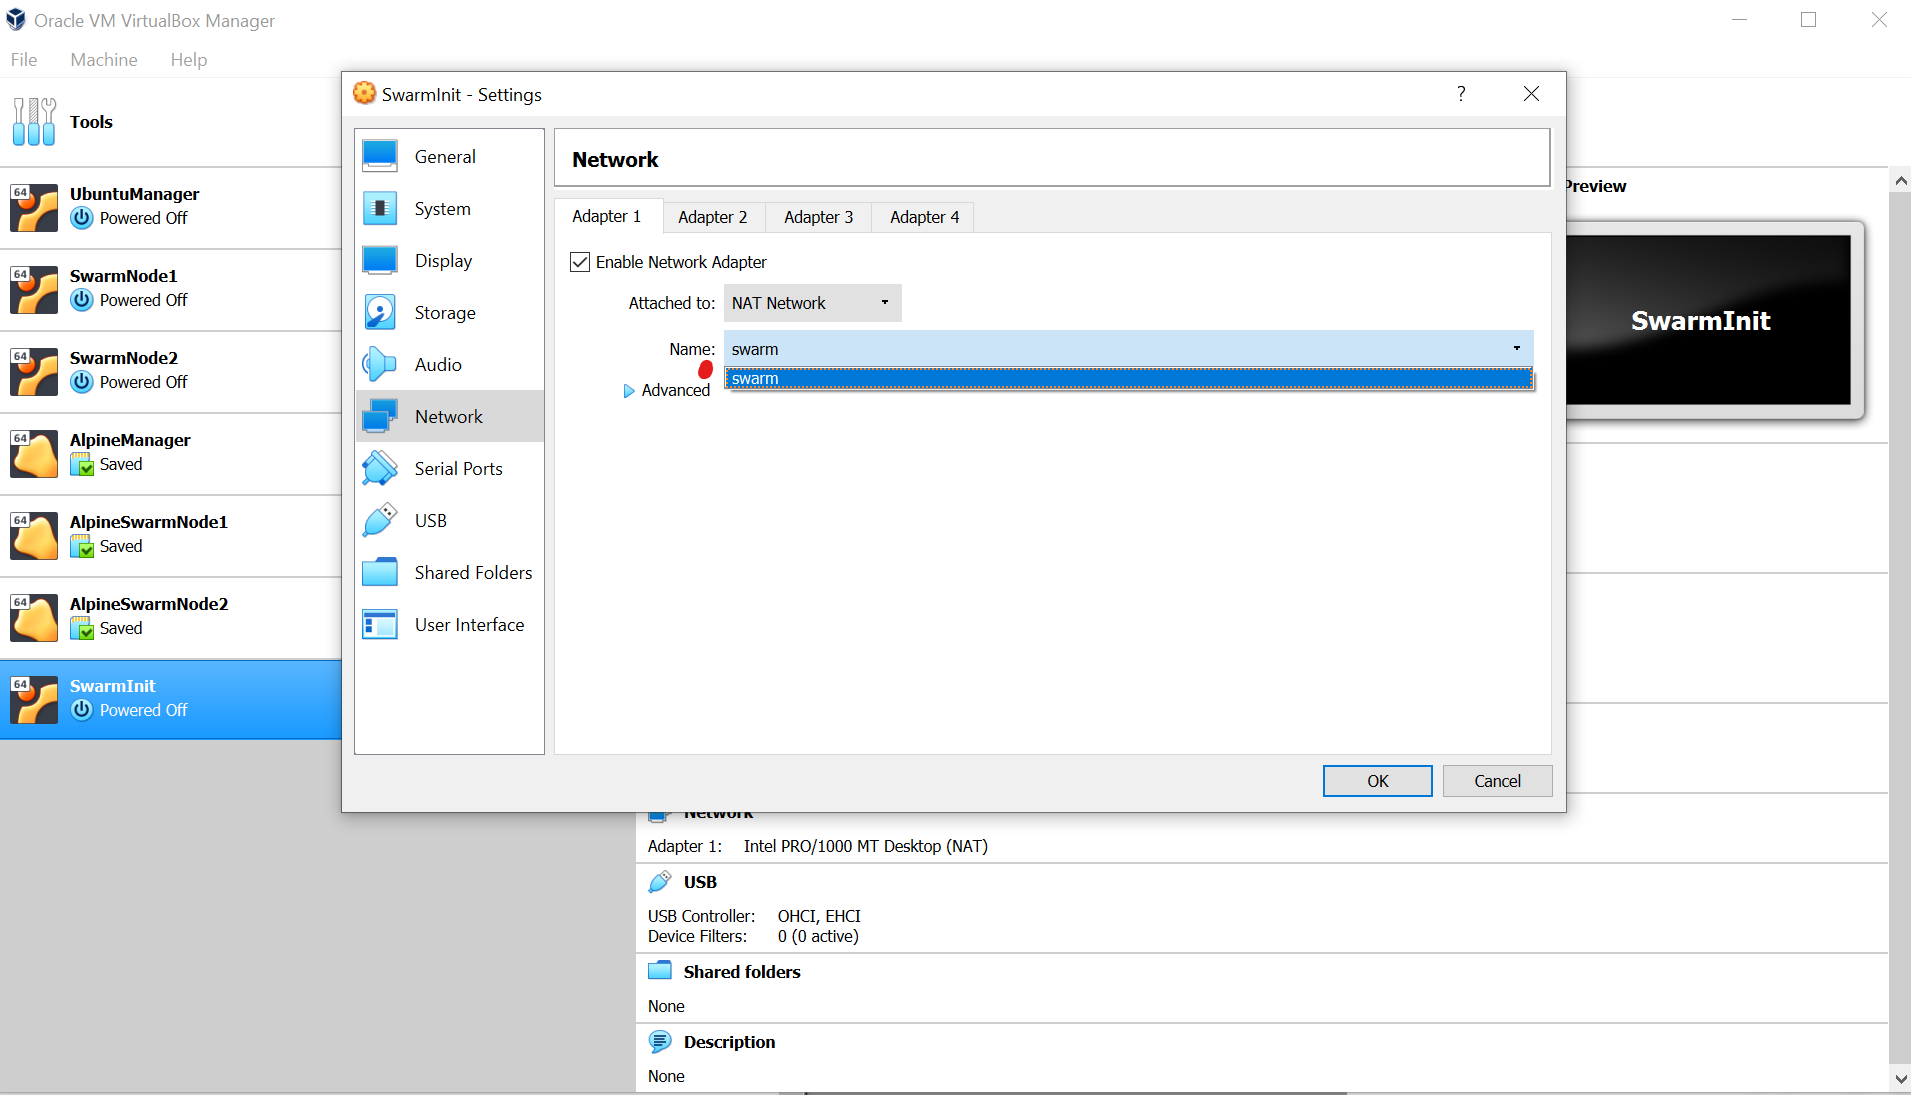
\includegraphics[width=\columnwidth]{./Figure/swarm-vm-init-net}
\end{center}
\end{frame}


\begin{frame}[fragile]
\frametitle{Swarm}
\framesubtitle{Setup: Initialize the Virtual Machine}
Attach to the \lstinline!Storage! cd-rom the \href{http://dl-cdn.alpinelinux.org/alpine/v3.9/releases/x86_64/alpine-virt-3.9.4-x86_64.iso}{AlpineLinux} iso. \\
\begin{center}
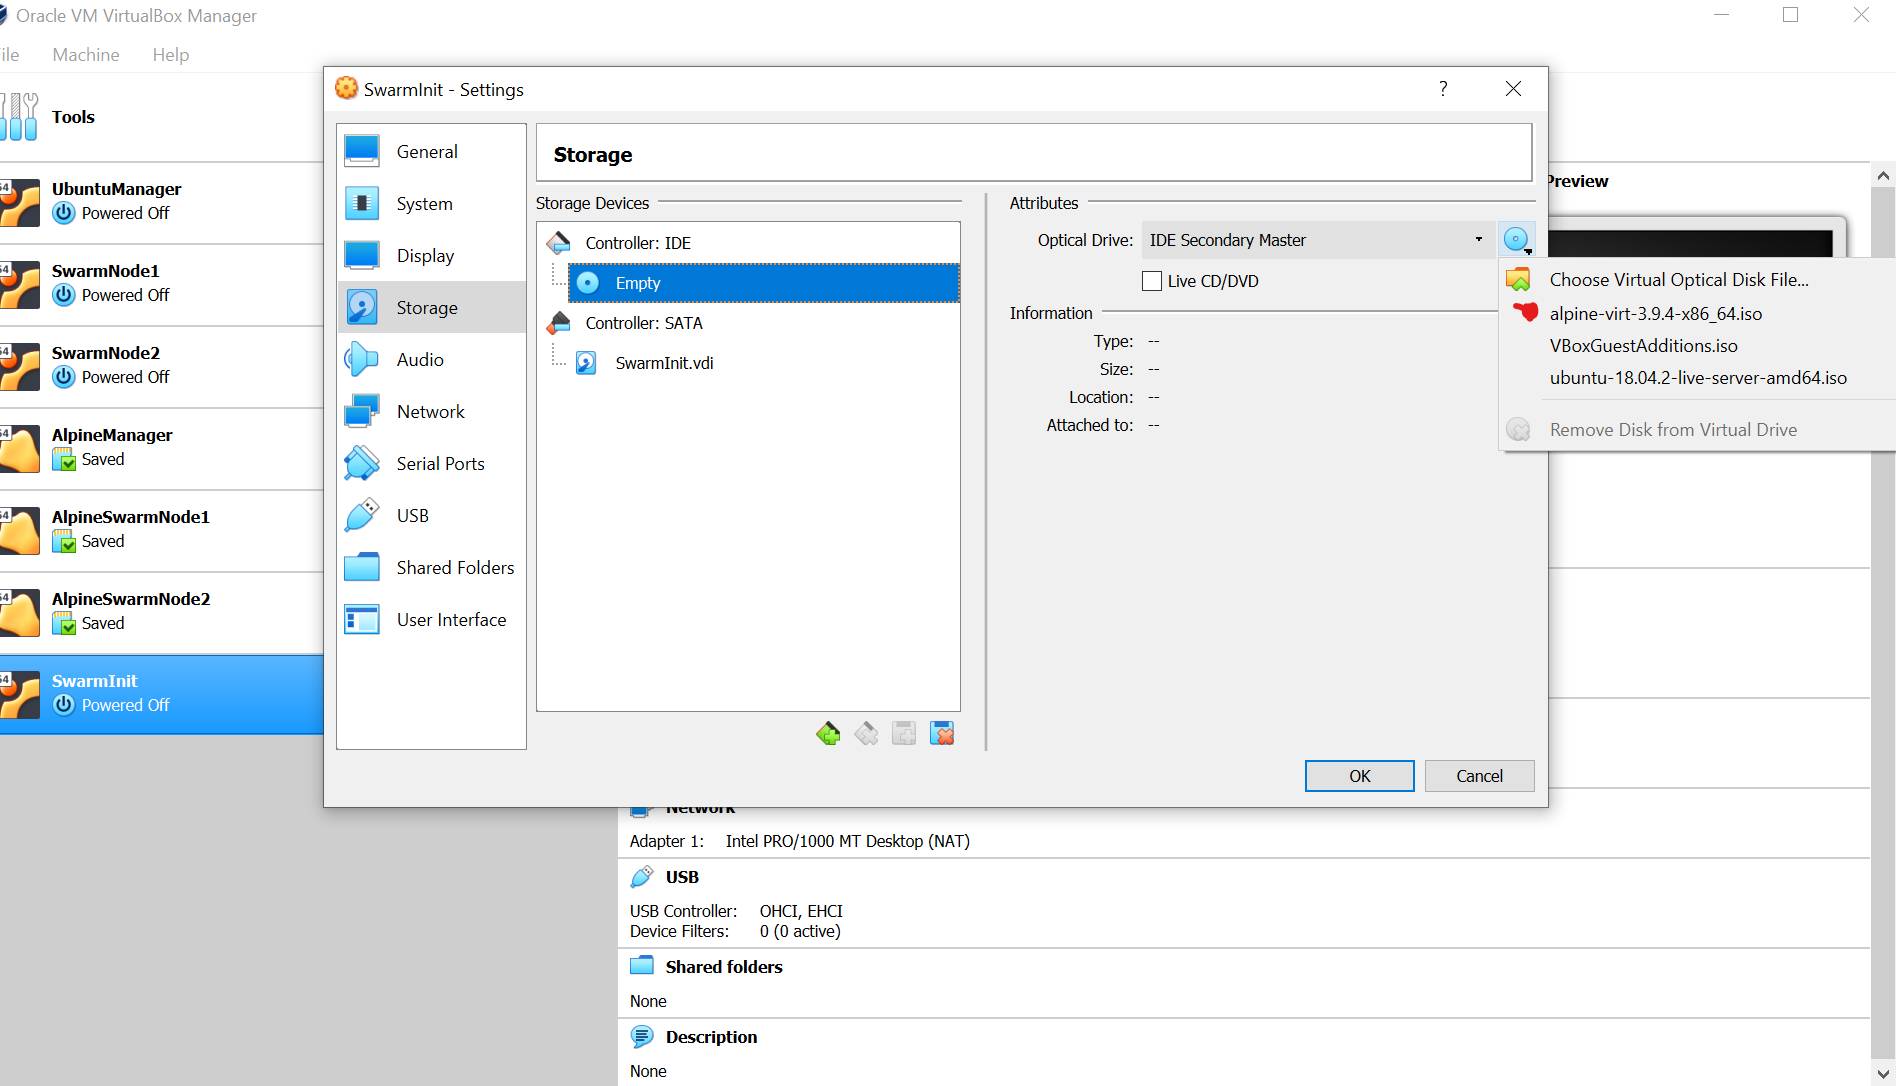
\includegraphics[width=\columnwidth]{./Figure/swarm-vm-init-cdrom}
\end{center}
\end{frame}

\begin{frame}[fragile]
\frametitle{Swarm}
\framesubtitle{Setup: Install AlpineLinux}
\begin{itemize}
\item Start the vm 
\item proceed with the installation procedure typing \lstinline!setup-alpine!
\item Set the network to \lstinline!DHCP!\\
\item Select the disk \lstinline!sda!
\item Select request mode \lstinline!sys!
\item \lstinline!reboot!
\end{itemize}
\end{frame}


\begin{frame}[fragile]
\frametitle{Swarm}
\framesubtitle{Setup: Install Docker into AlpineLinux}
\begin{itemize}
\item Start the vm
\item Login
\item 
\tiny
\begin{lstlisting}
echo"http://dl-cdn.alpinelinux.org/alpine/latest-stable/community" >> /etc/apk/repositories
\end{lstlisting}
\normalsize
\item \lstinline!apk update!
\item \lstinline!apk add docker!
\item \lstinline!rc-update add docker boot!
\item \lstinline!reboot!
\end{itemize}
\end{frame}


\begin{frame}[fragile]
\frametitle{Swarm}
\framesubtitle{Setup: Virtual Machines}
Do a full clone of the first machine creating 2 more.\\
\vspace{0.4cm}
For each clone regenerate the MAC address\\
\vspace{0.4cm}
Once logged into the machine change the hostname and reboot\\
\begin{lstlisting}
echo "SwarmNode1" > /etc/hostname
reboot
\end{lstlisting}

\begin{lstlisting}
echo "SwarmNode2" > /etc/hostname
reboot
\end{lstlisting}
\end{frame}


\begin{frame}[fragile]
\frametitle{Swarm}
\framesubtitle{Setup: Virtual Machines}
In every VM print the IP addess assigned by the DHCP. \\
\lstinline!ifconfig! \\
We need them to initialize Docker Swarm
\end{frame}